\ifsvnmulti
 \svnkwsave{$RepoFile: lyapunov/KS.tex $}
 \svnidlong {$HeadURL$}
 {$LastChangedDate$}
 {$LastChangedRevision$} {$LastChangedBy$}
 \svnid{$Id$}
\fi

\chapter{\KS}
\label{sect:LyapKS}

This section of the blog deals specifically with the
\KS\ calculations. General discussion is entered into
\refchap{c-DailyBlog} {Daily blog}.

% PC 2011-03-02: (b) generated by Kazz kaz2-PhysModes-b.png
\begin{figure}
 (a)~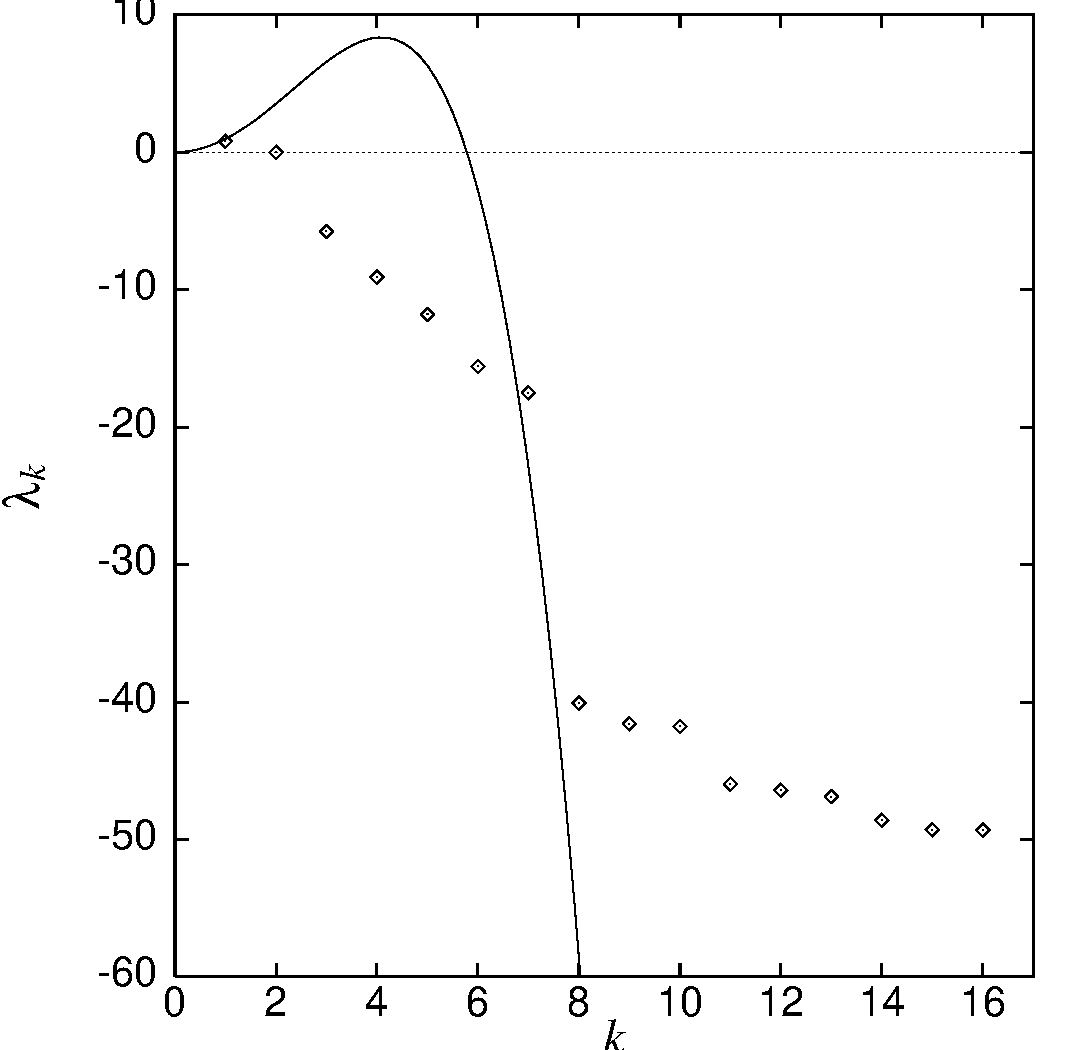
\includegraphics[width=0.40\textwidth]{eigenvalues}
 (b)~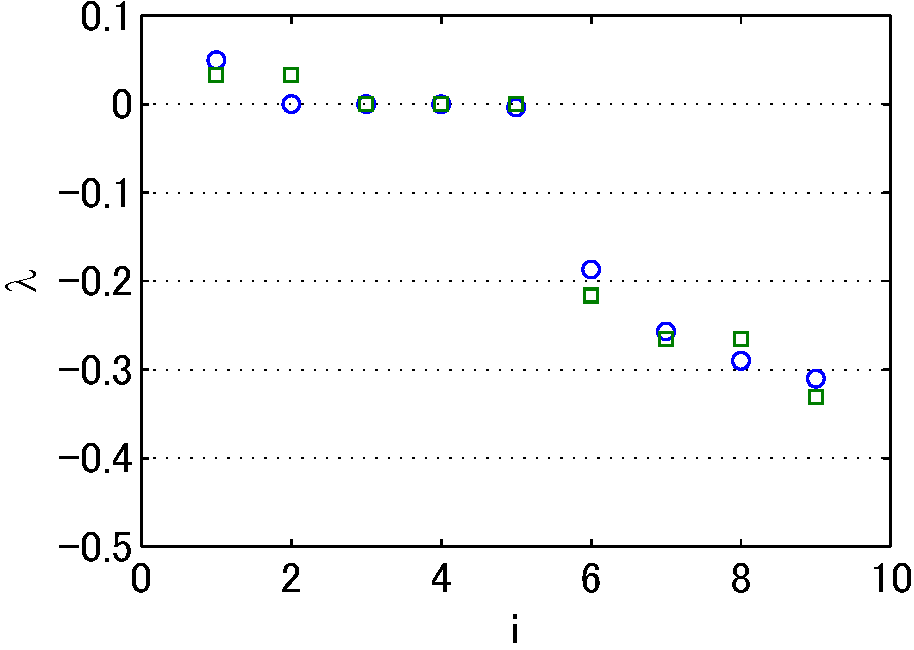
\includegraphics[width=0.50\textwidth]{kaz2-PhysModes-b}
\caption{
(a)
Lyapunov exponents $\lambda_k$ versus $k$ for the periodic
orbit $\overline{1}$ compared with  the stability eigenvalues
of the $u(x,t)=0$ stationary solution $k^2- \nu k^4$ (from
\refref{Christiansen97}). $\lambda_k$ for $k \geq 8$ fall
below the numerical accuracy of integration and are not
meaningful. Antisymmetric subspace,
hence no \SOn{2}\ pairing of eigenvalues, $N=16$ real Fourier
modes, $L=36.31$. One needs to rescale the time to compare
this to figure (b); -60 in the Lyapunov scale of figure (a)
corresponds to approx. -1.8 in \reffig{fig:lyapSpec}\,(a).
(b)
First 9 Lyapunov exponents $\lambda_j$ for the full
\statesp, periodic b.c. KS for $L=22$, from a 124 real Fourier
modes (blue circles) long-time simulation overlayed on
the $\period{p}=10.2534$ \po\ (green squares) [Kazz 2011-02-21].
}
\label{fig:lyapSpec1}
\end{figure}

% PC 2009-09-12: (a) generated by siminos/figSrc/gnu/lyapSpec.gnu
% PC 2011-03-02: (b) generated by Kazz kaz2-PhysModes-a.png
\begin{figure}
 (a)~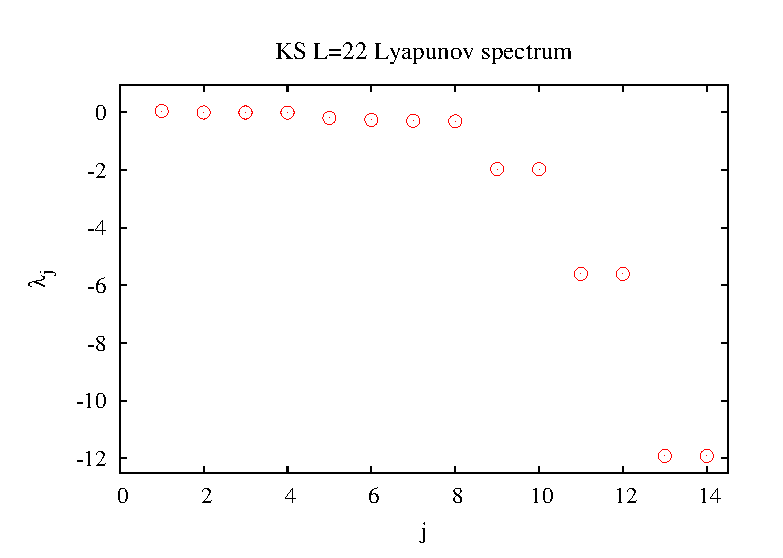
\includegraphics[width=0.48\textwidth]{lyapSpec}
 (b)~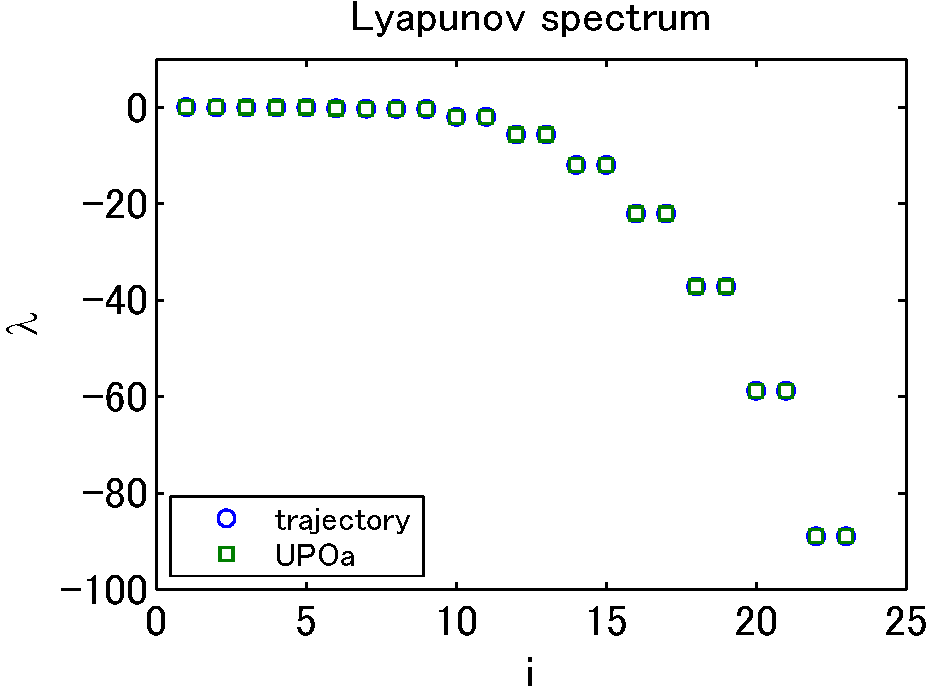
\includegraphics[width=0.42\textwidth]{kaz2-PhysModes-a}
\caption{
(a)
First 14 Lyapunov exponents $\lambda_j$ for the full
\statesp, periodic b.c. KS for $L=22$, from a 62 real Fourier
modes long-time simulation (from \refref{SCD07}).
(b)
First 24 Lyapunov exponents $\lambda_j$ for the full
\statesp, periodic b.c. KS for $L=22$, from a 124 real Fourier
modes (blue circles) long-time simulation overlayed on
the $\period{p}=10.2534$ \po\ (green squares) [Kazz 2011-02-21].
}
\label{fig:lyapSpec}
\end{figure}

\begin{description}
\item[2009-09-13 Predrag]
Sure looks persuasive, see \reffig{fig:lyapSpec}. I have also
added stability of a periodic orbit from
\refref{Christiansen97}, for KS on the periodic b.c.,
antisymmetric subspace, system size $\tilde{L} = 5.8$ close
to the onset of chaos, 16 real Fourier modes. As (perhaps?)
discussed in \refref{lanCvit07}, one has to be careful about
defining the effective system size $\tilde{L}$ for the
antisymmetric subspace, so these computations are done on
$L=36.31$ (or $L = 18.155$ if one considers the fundamental
$[0,L/2]$ domain only). Going from $(L,\nu) =
(2\pi,0.029924)$ of \refref{Christiansen97} to $(L,\nu) =
(L,1)$ convention used here requires that the time be
rescaled as $t \to \nu t$, and the Lyapunov exponents as
$\lambda_i \to \lambda_i/ \nu = \lambda_i/ 0.029924 $, so -60
in the Lyapunov scale of \reffig{fig:lyapSpec}\,(a)
corresponds to approx. -1.8 on the scale of
\reffig{fig:lyapSpec}\,(b), which would mean that then we
computed only the first pair of isolated eigenvalues. The
reason is that for periodic orbits we are computing {\em
Floquet multipliers} which underflow numerically very
quickly, so we cannot compute many {\em Floquet exponents}.
These covariant Lyapunov eigenvector methods are apparently
much smarter.

In \refref{lanCvit07} computations are done at $L = 38.5$,
but we listed only 4 eigenvalues per periodic orbit, and
considering hopeless organizational skills on the Lan astral
plane, I doubt that the full spectra can be rescued from
Lan's calculations. And, as explained above, probably we cannot
compute them for periodic orbits.

\item[Ruslan]
 Here's the expanded list of Lyapunov exponents for KS with $L = 22$:
 0.048,    0.0,    0.0,   -0.003,   -0.189,   -0.256,   -0.290,   -0.310,
-1.963,   -1.967,   -5.605,   -5.605,  -11.923,  -11.923...
So, there appears to be 8 `physically relevant' exponents and
the rest are pairs of hyperbolically separated ones.

I read
the papers about these covariant Lyapunov vectors and I'm not
sure I understand how they are related to eigenvectors at
periodic orbits: are they aligned?  I suspect that not quite,
apart from the most expanding and the most contracting
direction, the rest are sitting somewhere within the
subspaces spanned by the $k$ most expanding, or $m$ most
contracting eigendirections, but not quite aligned with the
eigendirections themselves.  That's probably why they are
more appropriately called `Lyapunov vectors'.

\item[2009-09-14 Predrag]
The `covariant Lyapunov vectors' are indeed the (right,
non-orthogonal) eigenvectors of the \jacobianM\ \jMps, as
defined in ChaosBook, and coincide with Floquet eigenvectors
for a periodic orbit.

 \item[Ruslan] I use 32 complex Fourier modes, so the
truncated system has 62 degrees of freedom.  The Lyapunov
exponent calculation is standard (using Gram-Schmidt).  The
exponents are the same, independent of the method of
calculation.  I have not attempted to calculate the covariant
Lyapunov vectors. I'm pretty sure that
orthogonality between physical and isolated eigenvectors
applies, but have not checked.

 \item[Ruslan]
It's OK to I email Hong-liu
Yang\rf{YaTaGiChRa08}, ask him to rerun his covariant
Lyapunov vector spectrum for $L=22$, to see whether he agrees
with us.

 \item[Ruslan]
I have the 62 eigenvalues/eigenvectors for all the RPO/PPO
I've detected, but for the highly contracting eigenvalues
the straightforward calculation
suffers from the numerical noise. We need a
better method to compute Floquet multipliers. I have now
checked:   Looks like {Kurt Lust} has proposed one, but I
cannot get his paper on ``Improved Numerical Floquet
Multipliers''\rf{Lust01}. If you could
get it for me, it would be great.

\item[2009-09-13 Ruslan]
``Structure of characteristic Lyapunov
vectors in spatiotemporal chaos''\rf{PaSzLoRo09} states
that characteristic Lyapunov vectors ``reduce to the Floquet
eigenvectors for a periodic orbit'' and references Trevisan
and Pancotti\rf{TrePan98}, which I cannot get electronically.

\item[2009-09-14 Predrag]
I added abstracts of these papers to the reading list above.
The `covariant Lyapunov vectors' are indeed the (right,
non-orthogonal) eigenvectors of the \jacobianM\ \jMps, as
defined in ChaosBook, and coincide with Floquet eigenvectors
for a periodic orbit. For a flow they are defined at a given
\statesp\ point by going back and forward a finite, but
`sufficiently long' time $t$, and coincide with the Floquet
eigenvectors if the point is (relative) periodic. I believed
that for a PDE we cannot go backward, but was wrong; the do
it by using the segment of forward trajectory stored in
memory. The reason why one can get the Floquet {\em exponent}
for arbitrarily long orbit is that the multiplier for eigenvector
evolved in time is just a number, so taking its logarithm over
short time segments and
storing it is trivial, no underflow problems one would get if
one worked with the Floquet {\em multiplier}. So we should be able
to keep track of all 62 eigenvectors, redo it for 126 eigenvectors,
and compare with plots in \refref{YaTaGiChRa08}.
Ginelli \etal\rf{ginelli-2007-99} are the main
reference on the `covariant Lyapunov vectors.' They describe
the QR algorithm for computing Gram-Schmidt vectors (GSV) and
recovering the covariant Lyapunov vectors (CLV) from them.
What confuses me is that so far all papers refer to $\Lyap_j
= \eigRe_j + i \, \eigIm_j$ as purely real, and list only
$\eigRe_j$, but I guess that will be explained somewhere.

\item[2009-09-14 Predrag]
My initial \reffig{fig:lyapSpec} was not optimal; I have now
replotted it as in Fig.~4 of
Yang \etal\rf{YaTaGiChRa08},
agrees with their 'extensivity' plot for $L=96$ and $192$.

I prefer $x$-axis to be $j/\tildeL = 2 \pi j/L$, as in
\reffig{fig:lyapSpecRscld}.

I do not like the way they count eigenvalues:  due to the $\On{2}$
2-dimensional irreducible representations
one should group their $j,j+1$ pairs,
plot them as a single, two-valued $j$, as in
\reffig{fig:lyapSpecRscld}. What one chooses to pair for low
$j$ might be ambiguous, as the nonlinear interactions mix up
the $\On{2}$ 2-dimensional linearly irreducible representations.
Reploted as in our much ignored 1997 paper\rf{Christiansen97},
eigenvalues fall onto $ (2 \pi j/L)^2 - (2 \pi j/L)^4 $
\eqv\ $\EQV{0}$  stability curve.
The isolated `covariant Lyapunov vectors'
are damped by $-(2 \pi j/L)^4$. I worry that we will not have such
amicable divorce for plane Couette and pipe flows...

% PC 2009-09-14: (b) generated by siminos/figSrc/gnu/lyapSpec.gnu
\begin{figure}
 (a)~\includegraphics[width=0.50\textwidth]{YaTaGiChRa08fig4}
 (b)~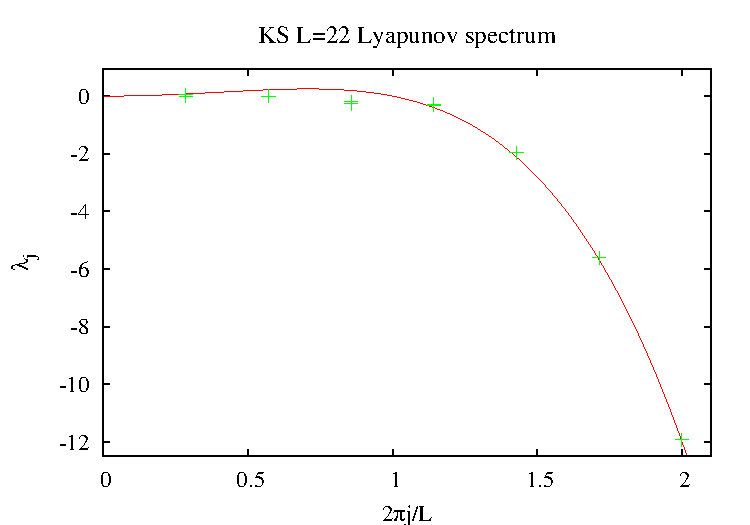
\includegraphics[width=0.40\textwidth]{lyapSpecRscld}
\caption{
(a)
Fig.~4 of
Yang \etal\rf{YaTaGiChRa08}:
Extensivity of the Lyapunov spectrum for the KS equation with
periodic b.c.. Inset: number of non-negative exponents (circles),
Kaplan-Yorke dimension (squares), metric entropy (diamonds,
multiplied by $50$), and number of physical Lyapunov vectors (triangles).
In perfect agreement with
\reffig{fig:lyapSpec}\,(b) here, plotted the same
(incorrect) way.
(b)
First 14 Lyapunov exponents $\lambda_j$ for the full
\statesp, periodic b.c. KS for $L=22$, from a 62 real Fourier
modes long-time simulation (from \refref{SCD07}).
The same as in part (a) and in \reffig{fig:lyapSpec}\,(b), but
abscissa is $j/\tildeL = 2 \pi j/L$, and each $j$ labels
the $\On{2}$ 2-dimensional irreducible representation
Lyapunov exponents pair.  Full line corresponds to
the stability eigenvalues
of the $u(x,t)=0$ stationary solution
$(j/\tildeL)^2- (j/\tildeL)^4$, for arbitrary system size $L$.
}
\label{fig:lyapSpecRscld}
\end{figure}


We also see
that the `physical' Lyapunov vectors are split into a less contracting 1/2
and more contracting 1/2 (different slopes in the
\reffig{fig:lyapSpecRscld}\,(a)). We
used to think the first 1/2 is the physically important one,
and say so in the arXiv version 2 of the article.
We stand corrected.

The Floquet eigenvectors of our (relative) periodic orbits are
what they call 'covariant,' so they should fit into their finite back/forth
time vectors like into a glove, whenever the respective state space
points are sufficiently close.

The main point of exploring the ergodic states space hierarchically
by periodic orbits is to tessellate it systematically, in the most
uniform way, by neighborhoods (linearized stable/unstable manifolds)
of periodic points. A periodic solution computed on a small system
size $L$, periodic b.c. is a solution on any multiple of $L$, and it comes
together with a smooth family of corresponding solutions for nearby
$L$'s.

I see prospects of a long and happy marriage here.

\item[2011-02-04 ES] Talked to Hugues Chat\'{e} and Kazumasa Takeuchi.
I was at CEA/Saclay for a thesis presentation today, bumped into Chat\'{e}
and
\HREF{http://daisy.phys.s.u-tokyo.ac.jp/student/kazumasa/}{Kazz}
(actually, it was more like invading their offices). Kazz updated me on
their latest work on Lyapunov vectors. We finally all agreed that we would give
the periodic orbit - Lyapunov vectors project a second try and arrange to meet
in Paris. I'll keep you posted.


\item[2011-02-07 ES] Sent Kazz an initial condition for a KS, $L=22$ \po\
with $\period{p}=10.2534$.

\item[2011-02-09 Kazz] I tried your initial condition and it works perfectly!
I also tried to calculate the Lyapunov exponents associated to this UPO.
The largest is about 0.03328, right? I'm not yet really sure about this value,
so it would be nice if you let me know the Lyapunov exponents you know for this UPO.

\item[2011-02-11 ES] The Lyapunov exponent I have is 0.033163, so you
are pretty close. In fact this exponent has multiplicity two, and
there is no other positive exponent for this orbit.

\item[2011-02-11 Kazz] Great! All you are saying (multiplicity, only two positive
exponents) are exactly what I confirmed with that UPO. I will soon have all
the necessary information regarding the physical/spurious Lyapunov vectors for that UPO.

\item[2011-02-11 Kazz] Which quantities / properties do you have
analytically / numerically for these UPOs in your methods? For instance,
if we know the time evolution operator for a UPO, we can compute both
Lyapunov exponents and covariant Lyapunov vectors as eigenvalues and
eigenvectors of that operator. Do you have them? Or, the exponent values
you have are just computed by Bennetin's standard algorithm?

\renewcommand{\ssp}{x}

\item[2011-02-11 ES] We do not use Bennetin's method, but rather
something similar to what you just described. However, I am not sure how
you exactly define the time evolution operator, so I will describe with
details what we do (see \refrem{rem:Lyapunov} on \refpage{rem:Lyapunov} above).

Given an initial condition $\xInit$ and period $\period{p}$ of the prime
\po\ $p$, we integrate
the differential equations for the nonlinear flow
$d\ssp/dt=v(\ssp)$, and a differential equation for the \jacobianM\
from $t=0$ to $\period{p}$,:
\beq
    \deltaX(t) = \jMps^t(\xInit) \deltaX_0
    \,, \qquad
\jMps^t_{ij}(\xInit)
  =  \left. {\pde \ssp_i(t) \over \pde \ssp_j} \right|_{\ssp=\xInit}
\, .
\label{hOdes1}
\eeq
\beq
{d\over dt}\jMps^t(\xInit)
    = {\Mvar}(\ssp) \, \jMps^t(\xInit)
\,, \quad
\mbox{initial condition~~} \jMps^0(\xInit) = \matId
\,.
\ee{Bew_Miaw}
The {\stabmat} (\velgradmat)
\beq
{\Mvar}_{ij}(\ssp) ={\pde \vel_i(\ssp)\over \pde \ssp_j  }
\ee{DerMatrix1}
describes the instantaneous rate of shearing of the infinitesimal
neighborhood of $\ssp=\ssp(t)$
by the flow.
We write for its
eigen\-vectors $\jEigvec[j]$
(sometimes referred to as `covariant Lyapunov vectors,'
or, for \po s, as `Floquet vectors')
\beq
\jMps_{p}(\ssp)\, \jEigvec[j](\ssp)
   = \ExpaEig_{p,j} \,\jEigvec[j] (\ssp)
\,,\qquad
\ExpaEig_{p,j}
= \sign{p}^{(j)} e^{\eigExp[j]_p \period{p} }
\,.
\ee{cplxExpaEig}
where $\eigExp[j]_p = \eigRe[j]_p \pm i\eigIm[j]_p$
and $\sign{p}^{(j)}$ are independent of
$\ssp$.
The time-dependent
$\period{}$-periodic vector fields, such
as the flow linearized around a \po, are
described by Floquet theory. Hence
we refer to a \jacobianM\
evaluated on a periodic orbit either as
a {\em \FloquetM} or a {\em monodromy matrix}, to its
eigenvalues
$\ExpaEig_{p,j}$ as Floquet multipliers,
% \refeq{cplxExpaEig},
and to $\eigExp[j]_p = \eigRe[j]_p+i\eigIm[j]_p$ as Floquet or
characteristic exponents.



The eigenvalues $\ExpaEig_i$ of $\jMps^t(\xInit)$ are
the Floquet multipliers and its eigenvectors the Floquet eigenvectors
(the covariant Lyapunov vectors for \po s).

Then the $i$th `Lyapunov' exponent is the real part
$\eigRe[i] = \ln(|\ExpaEig_i|)/ T$ of the Floquet exponent..
Although we only have the eigenvalues in file, I could easily compute
the eigenvectors for comparison.

The problem with this approach is that, while we believe the leading
eigenvalues to be accurate, the highly contracting ones suffer from
numerical noise. So it would be hard for us to separate physical from
isolated eigenvectors based on this computation alone.


\item[2011-02-11 Kazz] Thank you for the explanation. That is exactly what
I meant by eigenvalues of the time evolution operator.

I compute the Lyapunov exponents (and the covariant vectors)
by Benettin's method (and by Ginelli's one). The only trick is that, each time
the trajectory $\ssp(t)$ returns to its original position $\ssp(0)$, \ie, at every cycle
of the orbit, I replace $\ssp(t)$ by its initial value $\ssp(0)$. This is to kill
numerical noise that would grow and eventually kick the trajectory
out of the periodic orbit. This method is accurate even for very small
exponent values.

\renewcommand{\ssp}{a}

\item[2011-03-10 Predrag] That's OK for the shortest orbits, but
for longer orbits it will have to be replaced by either section $\to$
section traversals (see multi-shooting in
\HREF{http://chaosbook.org/paper.shtml\#cycles}{ChaosBook.org}) or variational methods (see
\refref{CvitLanCrete02} and
\HREF{http://chaosbook.org/paper.shtml\#relax}{ChaosBook.org}).

\item[2011-02-18 Kazz]

\BFIG{1.0}   % width=#1\textwidth
{kaz-evolution}   % f_name.pdf
{}   % short caption text
{    % full caption text
$\period{p}=10.2534$ \po\ [kaz-evolution]
}
{kaz-evolution}   % f-figure-label


Meantime I show you how my code integrates your UPO (the first three in your
list), \reffig{kaz-evolution}. Indeed, I cannot integrate
it even during one period for the second one, which has a large
Floquet multiplier.

by the way, the period indicated in the file is actually half the real period?
The space-time plot indicates that...

\item[2011-02-18 ES]

Yes, this is the convention we follow in our paper\rf{SCD07}, sorry for not
bringing this to your attention. We define the period $T_p$ to be the
smallest time such that $u(x+T_p)=\gamma u(x,0)$, where $\gamma$ a
discrete symmetry transformation (here reflection $R$), see eq. (2.22) in
our paper and the discussion that follows it. All periodic orbits we
have found are thus pre-periodic, or \rpo s.
\PC{really all are \rpo s? I thought about 1/2 of this 40,000 -
60,000 were not?}
The evolution
$T_p$ to $2T_p$ is a repeat of the pre-periodic orbit which
is periodic in this case, as $R^2=1$ (and thus we can take the period to be $T_p$
rather than $2T_p$). You should take advantage of this
when computing Lyapunov exponents, integrating only from $0$ to $T_p$ and
then applying $R$ to $u(x,0)$ to get a new initial condition, before
integrating from $T_p$ to $2T_p$ and so on. I should have mentioned this
convention, but it is by now second nature to me.

By the way, what method do you use for integration? For the third
orbit, could you please compute $||u(x,2T_p)-u(x,0)||$ (or
$||u(x,T_p)-Ru(x,0)||$ where $R$ is reflection)? The choice of norm should
not be crucial. I ask because I think this is the best indicator of
reproducibility of the periodic orbits. For the second orbit, if you
could compute $||u(x,T_p)-Ru(x,0)||$, it might tell us that the
difference is not as large as the figure suggests.

\item[2011-02-21 Kazz]

\BFIG{1.0}   % width=#1\textwidth
{kaz-evolution2}   % f_name.pdf
{}   % short caption text
{    % full caption text
$\period{p}=10.2534$ \po\ [kaz-evolution2]
}
{kaz-evolution2}   % f-figure-label


Thanks for the kind explanation. I should have read your
paper more carefully... I shall do this very soon.

Here I attach a figure, \reffig{kaz-evolution2}, showing
how a measure of the distance between a
trajectory and an orbit grows in time. The same trajectories and the orbits
as in the figure I send you last Friday are used. The dashed lines are the
growth rate expected from their Floquet multipliers and agree well with the
actual growth of the distance. Indeed, even for the second orbit the trajectory
stays close to it up to time $~2T_p$.

\item[2011-02-22 ES] In the last set of figures (evolution2.pdf), is $u(x,t)$
an orbit resulting from perturbing the initial condition of the periodic orbit?

\item[2011-02-23 Kazz] Concerning your question, the initial condition for u(x,t)
is exactly the one you sent to us. Just I integrated it and measured how
it deviates from the orbit because of the numerical noise.


\item[2011-02-20 Predrag] to Kazz:
I'm very glad that you and Evangelos are looking at the KS periodic solutions.
Attached is \refsect{sect:LyapKS} from out blog
(you probably have this already, but
I am not quite sure) - if you plot all cycle Floquet multipliers, can you try to
also plot them in the way suggested in my notes (it differs a bit from how you
had plotted them in Yang \etal\ paper\rf{YaTaGiChRa08})?
I was pleasantly surprised how well one
could see the physical/isolated boundary already for $L=22$.


\BFIG{1.0}   % width=#1\textwidth
{kaz2-PhysModes-cd}   % f_name.pdf
{}   % short caption text
{    % full caption text
Compare with frames (d) and (e) in \reffig{fig:lyapSpecCLG}.
$\period{p}=10.2534$ \po\ [kaz2-PhysModes-cd]
}
{kaz2-PhysModes-cd}   % f-figure-label

\BFIG{1.0}   % width=#1\textwidth
{kaz4-VectCompar}   % f_name.pdf
{}   % short caption text
{    % full caption text
$\period{p}=10.2534$ \po\ [kaz4-VectCompar]
}
{kaz4-VectCompar}   % f-figure-label

\BFIG{1.0}   % width=#1\textwidth
{kaz5-AngleTimeSeries}   % f_name.pdf
{}   % short caption text
{    % full caption text
$\period{p}=10.2534$ \po\ [kaz5-AngleTimeSeries]
}
{kaz5-AngleTimeSeries}   % f-figure-label

\SFIG{kazUPOa}   % width=#1\textwidth
{}   % short caption text
{    % full caption text
$\period{p}=10.2534$ \po\ [kazUPOa]
}
{kazUPOa}   % f-figure-label

\item[2011-02-21 Kazz]
I (with spirits of Hugues Chat\'e and Francesco Ginelli hovering above me)
have integrated some of
them and computed a number of quantities to elucidate the
physical/isolated separation of Lyapunov vectors. Here I show a
summary of preliminary results. I also have some questions to ask you
(see the end of the mail for them).


\textbf{Results}

Here we concentrate on (1) a ergodic trajectory generated from a random
initial condition, and (2) the first periodic orbit
$\period{p}=10.25336729174627$ in the list
Evangelos sent to me (called "UPOa" in the attached
figures). The numerical integration of the {unstable \po} is done by replacing the
trajectory on each period by the initial condition of the {unstable \po}.
    \PC{to Evangelos - do we have a naming convention in \refref{SCD09b}
        and/or \refref{SiminosThesis} that we could follow here,
        instead of renaming every \po? {\bf ES:} No. We use
	$(T_p,\ell_p)=(.,.)$ to refer to a \rpo.}

% PC 2011-03-02: (b) generated by Kazz kaz2-PhysModes-b.png
\refFig{fig:lyapSpec1}\,(b)
and
% PC 2011-03-02: (b) generated by Kazz kaz2-PhysModes-a.png
\reffig{fig:lyapSpec}\,(b)
show the Lyapunov spectrum for
the trajectory and the {unstable \po}.

For the {unstable \po} the exponents are
given by the Floquet multipliers, as indeed confirmed quantitatively,
while for the ergodic trajectory they are different from but close to
those of the {unstable \po}, \refFig{fig:lyapSpec1}\,(b).
 %(top right figure).
Increasing the index, we
see the appearance of the step-wise structure (top left figure) like in
our Yang \etal\rf{YaTaGiChRa08} PRL.

\refFig{kaz2-PhysModes-cd} shows the hyperbolic isolation of the physical and
isolated Lyapunov vectors (similar to frames (d) and (e) in \reffig{fig:lyapSpecCLG}
from our PRL); they
CANNOT be defined solely from the Lyapunov exponents.). The quality of
the data is not satisfactory because of the present length of the
simulation, but we can see that there are at most 11 physical Lyapunov vectors.


\refFig{kaz4-VectCompar} compares the covariant Lyapunov vectors on the
ergodic trajectory with the Floquet vectors of the {unstable \po}. I monitored the
ergodic trajectory and used the instant when it gets closest to the {unstable \po}
during the simulation. The inset of the top left figure shows the
snapshot of the trajectory (blue) and the {unstable \po} (red) at that instant.

The other three subpanels compare the vector structure at the same
instant. Here the spatial shift between blue and red is already taken
into account, so that you can directly compare the two profiles. The
bottom two figures show the 6th and 9th Lyapunov vectors, which correspond to
real-valued Floquet multipliers of the {unstable \po} (thus Oseledec subspace is
not degenerated). We can see that the vectors of the ergodic trajectory
become quite close to the {unstable \po} counterparts (but not exactly; some are
better, others are not as good). For the Lyapunov vectors that correspond
to complex conjugate pairs of the Floquet multipliers, e.g. 1st and 2nd
ones, we have to compare a vector of the trajectory with arbitrary
linear combinations of the 1st and 2nd {unstable \po} vectors. Indeed, we can find
a combination that gives a structure similar to the vector of the
trajectory.

In short, as a ergodic trajectory wanders among {unstable \po}s, the vectors of the
trajectory change their shape incessantly to follow the vectors of the
closest {unstable \po} at each instant.


Now, the question is whether we can unambiguously define the physical
and isolated Lyapunov vectors for each periodic orbit, or not. We don't know how to
do this, because the angle between any Lyapunov vectors
of {unstable \po} varies periodically and thus does not reach 0 or
$\pi$ forever.

Moreover, we find that the hyperbolicity properties crucially depend on
the quality of the periodic orbit. See
\reffig{kaz5-AngleTimeSeries}, which shows
time-series of angles between given pairs of the Lyapunov vectors of the
{unstable \po}. Although the angle between Lyapunov vectors of index $\geq 11$ (correspond
to isolated Lyapunov vectors for the ergodic trajectory) stays close to $\pi/2$ with a
seemingly trivial time-evolution, the numerically computed angle is not
strictly $\pi/2$ and is subject to a very slow convergence (see the middle
panel). To test, I added a noise to the initial condition of the {unstable \po} and
computed the same quantities. While the angles for index $\leq 10$ do not
show significant changes, those for index $\geq 11$ show spurious
oscillations with long periods.

This is why we think that the quality of the periodic orbit is crucial.
It could be that, if we had an initial condition with infinite
precision, the angle for index $\geq 11$ are strictly orthogonal, and thus we
could define the isolated Lyapunov vectors from this strict orthogonality.


\textbf{Questions}

1) We wonder if we may define the physical and isolated Lyapunov vectors for
periodic orbits. Do you have any ideas, in particular from the viewpoint
of the Floquet multipliers and eigenvectors?

2) As shown above, the quality of the {unstable \po} initial conditions turns out
to be crucial. Do you have data with better resolutions? Or, is it
numerically difficult to compute {unstable \po}s with very high resolutions?

That's all for now. Any comments / questions are of course welcome!


\textbf{Kazz to Predrag} I made a plot of the Lyapunov spectrum of
the {unstable \po} (the same one as above) in the same way as you did. See \reffig{kazUPOa}
and UPOa-lyap.dat (below). I hope this is the one you wanted.

                            \noindent
 3.3274529258200000e-2    \\
 3.3273022876699997e-2    \\
 1.2294744377000001e-5    \\
 -1.3236540275600000e-5    \\
 -7.2634814842399998e-5    \\
 -2.1629227416399999e-1    \\
 -2.6517234146000002e-1    \\
 -2.6516527982799998e-1    \\
 -3.3072168309500000e-1    \\
 -1.9602739059100001    \\
 -1.9673554279600001    \\
 -5.6025023421000002    \\
 -5.6042396292200003    \\
 -1.1925106699200001e+1    \\
 -1.1925523679299999e+1    \\
 -2.2011597078699999e+1    \\
 -2.2011657848500001e+1    \\
 -3.7116197744200001e+1    \\
 -3.7116202659300001e+1    \\
 -5.8760926784699997e+1    \\
 -5.8760926787599999e+1    \\
 -8.8935807811399997e+1    \\
 -8.8935807884699997e+1    \\

\item[2011-03-05 Predrag to Kazz] I do not understand your \po\ calculations.
For this short orbit I expect everything - all Floquet multipliers and
Floquet vectors to be good to a machine precision, or at least to - let's say -
$10^{-6}$?

\item[2011-03-05 Predrag]
I find
\reffig{fig:lyapSpec1}\,(b) amazing. The $\period{p}=10.2534$ \po\ is
only exploring the $\infty$-dimensional \statesp\ as the
shortest 1-dimensional loop, while the ergodic trajectory is
wondering over the whole 11-dimensional (say Parisians) strange attractor
(inertial manifold) and still the entangled eigenvalues are so close.

\item[2011-03-07 Hugues]
That's because the $\period{p}=10.2534$ \po\ is the least unstable of all
\po s.

\item[2011-03-07 Predrag] Easy to say, but in \refref{SCD07} we have
not noticed any concentration of the natural measure in the neighborhood of
this \po. That is perhaps because we have not quotiented
$\pS \to \pSRed = \pS/\SOn{2}$, and $\SOn{2}$ drifts can easily
mask a much simpler strange attractor\rf{SiCvi10,FrCv11}.


\item[2011-03-04 Evangelos]
I really can't follow this tessellation idea. My motivation to be
involved with this project at this point developed while reading Roweis
and Saul\rf{RoSa00}. I believe what we ought to do should be very close
to their way of thinking: construct linear local charts (bases) and then
bring them together to construct a global curvilinear embedding. In
contrast to their pattern recognition, empirical way to construct the
local charts, we can use information from the covariant Lyapunov vectors.

\item[2011-03-05 Predrag]
I agree in principle.

\item[2011-03-04 Evangelos]
I would prefer to work with \KS\ in the antisymmetric subspace, so that we do not
have to worry about the translational symmetry (remember that the periodic
orbits for $L=22$ are in the full space, rather that in the antisymmetric
subspace).

\item[2011-03-07 Hugues]
I agree, shifts are killing us.

\item[2011-03-05 Predrag]
I agree.
    \PCedit{
[revised 2011-03-10: I disagree, see comment below]
    }


\item[2011-03-04 Evangelos]
The local charts can be provided by the physical covariant Lyapunov
vectors computed on a set of the most important \po s. Then we only need
to implement the final step in the procedure of Roweis and
Saul\rf{RoSa00}, which involves solving a minimization problem for the
global coordinates and should be computationally tractable if a truly
low-dimensional embedding exists.

\item[2011-03-05 Predrag]
We cannot tessellate with \po s; we can only work with \emph{periodic
points}, hence we need to understand what Floquet vectors (AKA `covariant
Lyapunov' vectors evaluated on \po s) tell us about the `physical
dimension' of the local \Poincare section.

\item[2011-03-04 Evangelos]
How could a trajectory be confined to a \Poincare section? You seem
to talk about local charts in \refsect{sec:chart}, rather than \Poincare sections.

\item[2011-03-05 Predrag]
Ant is not following a \emph{trajectory}, ant is moving \emph{transversely}
to the time flow, for example: if the continuous time trajectory has one
unstable eigen-direction, it sweeps out a 2-dimensional unstable manifold,
whose \Poincare section is 1-dimensional curve that the ant could follow.

\item[2011-03-04 Evangelos]
If we manage to use local \Poincare sections to reduce the flow to a
discrete map (or maps) before applying this procedure, we would then only
need one (or a few) representative point(s) per periodic orbit for our
local charts, rather than points along the full orbit. However, we know
this is tricky to do in a high-dimensional space, before an embedding is
available.

\item[2011-03-05 Predrag]
\HREF{http://en.wikipedia.org/wiki/String_Quartet_No._16_(Beethoven)}
{Es muss sein!} No sense can be made out of a collection of \po s unless
they and their Floquet vectors are reduced onto  \Poincare sections.

\item[2011-03-04 Evangelos]
In any case, while I can see many local \Poincare sections working
together, either before or after the global coordinates are found, I
cannot see how a tessellation as you describe it here would work.
\Poincare sections are designed to pierce the flow (so the ant we follow
would leave the section immediately) and good sections should be
transverse, not tangent to the attractor.

\item[2011-03-05 Predrag] Grave misunderstanding. The continuous group
that is being reduced by \Poincare sections is the evolution in time.
After the reduction of continuous time to discrete time, what remains are
the affine hyperplanes (local \Poincare sections) which are
\emph{tangent} to the strange attractor; the ant is not crawling in the
time direction, she is crawling (for example) along the unstable manifold
heteroclinic section as it is seen within the \Poincare sections, not the
time trajectory traced out in the full \statesp.

\item[2011-03-02 Evangelos] First meeting's wisdom:
\begin{itemize}
 \item[2011-03-02 Parisians] We
 \HREF{http://en.wikisource.org/wiki/Gargantua/Chapter_XVI}{Parisians}
  all agree that it's best to work on antisymmetric subspace KS.

\item[2011-03-10 Predrag]
    \PCedit{
I'm very worried about this development. We have settled in \refref{lanCvit07}
on $L=22$ as the smallest system size for which
the translationally invariant KS
is empirically `shmurbulent.' We cannot work with
\KS\ in the antisymmetric subspace at $L=22$, because there is no chaos there
- that's why Lan and I worked\rf{lanCvit07} at  $L = 38.5$. We cannot work with
\KS\ with the fixed $u(0)=u(L)=0$ boundary conditions at $L=22$,
because there will be no shmurbulence there either - when the ends are pinned down, one needs a larger cell to approach the onset of shmurbulence,
that's why the antisymmetric subspace required going up to $L = 38.5$.
Besides, for small $L$ the boundary effects will dominate the dynamics,
the \statesp\ geometry will be very different, and
what we learn there will not scale to larger $L$. What was so elegant
about analysis\rf{SCD07} of  $L=22$ system is that the geometry of
the \statesp\ was so much more beautiful than what it is for the
$L = 38.5$ antisymmetric subspace. Since then we have lost fear of
continuous symmetries\rf{SiCvi10,FrCv11}. And continuous symmetries are the physically interesting case.
In summary, going to fixed b.c. is ugly, unphysical, and to add insult
to injury, it would necessitate a whole new fishing expedition,
abandoning all the wisdom we already have in the $L=22$ case.
    } %end \PCedit{


\end{itemize}



\item[2011-03-02 Evangelos] First meeting's numerics:
\begin{itemize}
 \item Evangelos will do the shooting for periodic orbits
	(we need to decide on system size). He hopes he will find the time \ldots
 \item Kazz uses an implicit second order Adams(-Moulton) method (see post of
	2011-03-09), with pseudospectral space discretization.
	He uses some prescription for anti-aliasing, in order to keep the large wavenumbers
	and corresponding isolated Lyapunov vectors uncontaminated. Uses numerical
	recipes for FFT. (ES suggests switching to FFTW as numerical recipes FFT is
	known to be unreliable in double precision.)
 \item Evangelos uses explicit fourth order Runge-Kutta with exponential
	time differencing (see \refref{ks05com}) and pseudospectral space
	discretization. He uses brute force anti-aliasing (increases resolution
	to the point that only Lyapunov vectors already at round-off are affected by
	aliasing). He uses FFTW.
 \item We agreed that a good strategy would be that Kazz implements a simple
	Newton routine, so that he can refine the orbits I give him. I've
	pointed him to Chaosbook chapters, my own first year report on Newton's
	method for periodic orbits and my thesis.
 \item I've also agreed to give Kazz the backbone of my integrator routines
	(and also pointed him to \refref{ks05com}). Kazz is suspicious towards
	Trefethen's algorithm, he thinks that the integrating factor trick might
	lead to under-resolved large wavenumbers and problematic isolated
	Lyapunov vectors (and that the implicit method performs better in this
	respect). I can't argue in favor of one or the other integrator.
 \item I am also thinking to try to implement anti-aliasing and see
	if agreement improves.
\end{itemize}

\item[2011-03-09 Kazz] to Evangelos:
Before your mail I made a code to improve the quality of the periodic orbits
and it works very well. Now, with my integrator, the norm of distance
(with square root) after one cycle is on the order of $10^{-13}$ for the orbit
I focus on, and the trajectory stays nearby over $40$ periods, to be compared
with $10$ for the original orbit data. I restarted all the calculations
with this improved orbit.

To answer your question, my code uses the splitting method with the
2nd-order implicit method
\HREF{http://en.wikipedia.org/wiki/Linear_multistep_method}{(Adams-Moulton)}
for the linear terms and the 2nd-order Runge-Kutta
\HREF{http://en.wikipedia.org/wiki/Heun\%27s_method}{(Heun method)}
for the nonlinear term.

For the aliasing, I use at least $(3N+1)$ spatial points when computing
the nonlinear term, where $N$ is the wavenumber cutoff of the Fourier modes.
Under this condition the pseudospectral method is exact
(equivalent with the spectral method apart from the computational cost).

\BFIG{1.0}   % width=#1\textwidth
{kaz-fig-temp}   % f_name.pdf
{}   % short caption text
{    % full caption text
$\period{p}=10.2534$ \po\ [kaz-fig-temp]
}
{kaz-fig-temp}   % f-figure-label

\item[2011-03-10 Kazz] To refine the orbits I use Newton's method,
but I adapted it to apply to half a period, playing with the reflection
symmetry. That is to say, instead of considering
\[
  (I-J(u))(u'-u) - vt = -(u-f(u))\,
\]
I use
\beq
  (R-J(u))(u'-u) - vt = -(Ru-f(u))\,
\ee{eq:preper-newt} where $R$ is the operator
for the reflection, i.e., $Ru(x) = -u(-x)$.
It is better, not only because the integration time is half, but also because
the reference coordinate $x_0$ for the reflection $u(x,t)=-u(x_0-x,t+T_p)$
is automatically set to be 0.

That said, I looked at the results from the refined orbit, and found
that the results do not change. The angle between spurious Lyapunov vectors oscillates
always with a finite amplitude.

\item[2011-03-10 ES] My bad here, I forgot to mention to Kazz that we
use \refeq{eq:preper-newt} for pre-periodic orbits \ldots

\item[2011-03-10 Ruslan] {\em Comment on the numerical approximation of the KS flow}\\
I would suggest not to worry too much about the accuracy of the numerical approximation of the KS flow.  Instead, it is better, in my opinion, to adopt the viewpoint that one investigates the properties not of the KS flow, but of the map defined by the numerical integrator of the \KSe, which approximates the solutions of the \KSe.  As long as the orbits of the map resemble the solutions of the flow (think of it in terms of shadowing), the results of our investigation of the map will faithfully represent those for the KS flow.  So, it doesn't matter whether one investigates the Kassam-Trefethen map or the Adam-Moulton-RK map: the qualitative picture will be the same.

The neat thing about Kassam-Trefethen map is that it solves the linear part of the KS flow exactly, thus eliminating the problem of the stiffness of the linear part, and thus allowing to use a much larger time step.  Implicit Adams-Moulton also deals with the stiffness, but it solves the linear part only approximately, so it is likely to be less accurate if used with the same time step.

From the same viewpoint, there is also no need, in my opinion, to use anti-aliasing.  If a better approximation of the KS flow is needed, just include more modes into the map and decrease the time step.  Of course, if Kazz already implemented anti-aliasing, then there is no harm in using it, provided it doesn't increase the flops count too much.

\item[2011-02-21 Kazz]
If the isolated Lyapunov vectors of
{unstable \po}s are strictly orthogonal, it means that the \jacobianM\ for a
cycle can be decomposed to two parts, one of which would be an
orthogonal submatrix. Does that seem likely to you?

\item[2011-03-10 Ruslan]
I don't see why we should expect higher Lyapunov vectors to be {\em exactly} orthogonal.  Since all Lyapunov vectors in the \KSe\ are coupled though the nonlinear term, the deviation from orthogonality should be proportional to the strength of this coupling.  Of course this coupling is very weak for higher Lyapunov vectors and decreases exponentially with increasing mode number.  But if we measure with sufficient resolution, which is what Kazz does, we'll observe the deviation from orthogonality for any higher mode, whether anti-aliased or not.  Or am I wrong?

\item[2011-03-10 Predrag] My belief too. There is no reason to require non-physical Floquet vectors to be pure, orthogonal Fourier modes: all
    we need is that perturbations along these directions are pushed back into
    the attractor without being entangled along it...

\item[2011-03-11 Ruslan] It seems to me that the behavior of the isolated Lyapunov vectors in the \KSe\ is rather easy to understand.  Since they are essentially generated by the linear part of the \KSe, they will be nothing else but the Fourier modes living in mutually orthogonal planes.  That is, they are the eigenvectors of the \jacobianM\ of the trivial equilibrium $u = 0$, just slightly perturbed by the nonlinear coupling.  But since, as I already said, this perturbation decays exponentially with the mode number, it is negligible for high enough modes.  So, to answer Kazz's question, the strongly contracting eigenvectors of the \jacobianM\ of a cycle should be essentially orthogonal to one another as well as to the subspace spanned by the expanding and weakly contracting eigenvectors (i.e. the subspace where the physical Lyapunov vectors live).

\item[2011-06-28 Evangelos]
Met with Kazz at \HREF{http://cct11.cpt.univ-mrs.fr/}{CCT11 conference}
at Marseilles and discussed about their progress with Lyapunov vectors
for periodic orbits. To my understanding, the main points are: Kazz
\etal, identify generic orbits that come close to a periodic orbit. They
use the vector defined by the points of minimal distance along these two
trajectories as a local approximation to the ``inertial manifold.''
However, some of the Lyapunov vectors computed along the periodic orbit
and the generic trajectory are not identical or even similar (at the
points of minimal distance). Kazz argues that it is not possible to
define physical and isolated modes for periodic orbits (in his numerics
the number of physical dimensions inferred from a periodic orbit would
be, in general, different from the number of physical dimensions inferred
from a generic orbit).

\item[2011-06-28 Predrag] I will deal with this in bits:
First, not being in frequent contact is not working for me - I
do not know what is being computed or why. Are we in the \KS\
antisymmetric subspace at\rf{lanCvit07} $L = 38.5$, or the
full space at $L=22$? As I wrote above in the {\bf 2011-03-10}
entry, I believe we cannot work in the \KS\ antisymmetric
subspace at $L=22$, as there is no shmurbulence there. If Kazz
is integrating trajectories in the full space at $L=22$, he
\emph{must} quotient the translational $\SOn{2}$, otherwise
there is no way to define the (locally minimal) Euclidean
distance(s) between a \po\ and a generic long-time trajectory\rf{FrCv11}.

\item[2011-07-22 Evangelos] Spatial shift in eq. (2) of 2011-07-21 draft seems
to take care of that, although this approach seems to be somewhat inefficient.
A question: Is the spatial shift a multiple of the spatial discretization step?
If yes, then this means that you probably overestimate the distance of minimum
approach based on eq. (2). You should then refine the comparison by introducing
a local slice as in \refrefs{SiCvi10,FrCv11}.


\item[2011-06-28 Predrag]
Using ``the vector defined by the points of minimal distance along these two
trajectories as a local approximation to the inertial manifold'' makes no sense to me.
The local approximation to the inertial manifold is spanned by the transverse
\po\ Floquet eigenvectors at that periodic point (simplest to take a local \Poincare section
normal to $\vel(\ssp)$ at $\ssp$).

\item[2011-06-28 Predrag]
If the generic trajectory is close the periodic point in a direction
along its unstable manifold, it is close. If it belongs to a different fold of the
unstable manifold, than it is far away and can have quite different local
tangent space.

If the two points are close, the periodic point tangent space
eigen-directions should be close to the covariant vectors at the nearby generic
point, as they are probing the same stable / unstable manifolds structure in the
linear neighborhood that includes them both.

\item[2011-07-22 Evangelos]
I've actually raised the objection about the generic trajectory belonging to a
different fold of the unstable manifold of the periodic orbit to Kazz in our
discussion at Marseilles. His
counter-argument is, I think, based on figure 5(c) of 2011-07-21 draft. His
claim is that since the angle tends to zero as the generic trajectory approaches
the periodic orbit the approach has to be along the unstable manifold.
However, I am not convinced that we can numerically tell the difference
if the minimum distance along the local unstable
eigen-direction is much larger than the separation of folds of the unstable
manifold. Kazz, could you please clarify and give as more insight?

\item[2011-06-26 Kazz] It is not possible to
define physical and isolated modes for periodic orbits (in my numerics
the number of physical dimensions inferred from a periodic orbit would
be, in general, different from the number of physical dimensions inferred
from a generic orbit)

\item[2011-06-28 Predrag]
A short \po\ might be quite hyperbolic, \ie\ never get close to any
tangencies (small angles between leading Floquet eigenvectors). The longer ones
should probe heteroclinic tangencies a bit better...

\end{description}
